\documentclass[12pt, danish]{beamer}

\usepackage[danish]{babel}
\usepackage[utf8x]{inputenc}
\usepackage{graphics}
\usepackage{srcltx}
\usepackage{float}
\usepackage{layout}
\usepackage{listings}

\title{Topics in Programming Languages}
\author{.. \& Mads Hartmann Jensen}

\mode<presentation>
{
  \usetheme{Frankfurt}
  %\usetheme{Warsaw} 
  \definecolor{uofsgreen}{rgb}{.125,.5,.25}
  \definecolor{natvidgreen}{rgb}{.196,.364,.239}
  \definecolor{kugrey}{rgb}{.4,.4,.4}
  \usecolortheme[named=uofsgreen]{structure}
  \usefonttheme[onlylarge]{structuresmallcapsserif}
  \usefonttheme[onlysmall]{structurebold}
}

\usenavigationsymbolstemplate{} % fjern navigation

\setcounter{tocdepth}{1}

\def\height{0.6\paperheight}
\def\width{0.9\linewidth}

\setlength{\marginparwidth}{1pt}
\setlength{\hoffset}{1pt}

\begin{document}

\begin{frame}
\titlepage
\end{frame}

\section{Eden}

\subsection{What}

\begin{frame}
\frametitle{What is Eden?}

Eden is a parallel functional programming language which extends
Haskell with constructs for the definition and instantiation of
parallel processes.\\
\pause
So what's new?
\end{frame}

\begin{frame}
\frametitle{Eden is distributed}

\begin{itemize}
\item Eden is designed for \textbf{distributed-memory} machines
  (clusters).\pause
\item This means \textbf{message-passing}, no shared memory.\pause
\item Very suitable paradigm for functional programming.\pause
\item Even better: very suitable for the Par monad!
\end{itemize}
\end{frame}

\begin{frame}[fragile]
\frametitle{Processes as functions}

\begin{verbatim}
process :: ( Trans a , Trans b ) =>
  (a  b) -> Process a b
( # )   :: ( Trans a , Trans b ) =>
  Process a b -> a -> b
\end{verbatim}
\pause
\begin{verbatim}
fib :: Int -> Int
fib 0 = 1
fib 1 = 1
fib n = process fib # (n-1) + process fib # (n-2)
\end{verbatim}
\end{frame}

\begin{frame}[fragile]
\frametitle{Eden skeletons}

Eden provides skeletons for parallel processing tasks.

\begin{verbatim}
parMap :: ( Trans a , Trans b ) =>
          ( a -> b ) -> [ a ] -> [ b ]
parMap f = map (process f #)
\end{verbatim}
\pause
\begin{verbatim}
farm :: ( Trans a , Trans b ) =>
        ([a] -> [[a]]) ->       -- ^ distribute
         ([[b]] -> [b]) ->      -- ^ combine
         (a -> b) -> [a] -> [b] -- ^ map interface
farm distribute combine f
  = combine . ( parMap ( map f )) . distribute
\end{verbatim}
\pause
We don't make use of this.
\end{frame}

\subsection{How}

\begin{frame}
\frametitle{Structure of Eden}

\begin{figure}
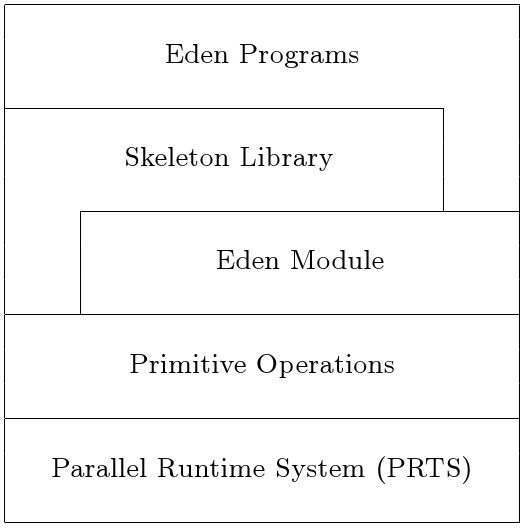
\includegraphics[width=5cm]{edenstructure.png}
\end{figure}

Supports PVM and MPI middleware.

We use EDI, the Eden Implementation Language, a type-safe wrapper
around the primitive operations.
\end{frame}

\begin{frame}
\frametitle{Conceptually}

A \textbf{channel} connects the outport of a thread with an inport of
a receiver thread.  The channel consists of a writing end and a
placeholder for reading.

\pause

A channel can be a \textbf{stream} (list), where elements are sent
one-by-one.

\pause

Each machine runs a process, consisting of multiple threads, with a
one-to-one relation between threads and outports.

\pause

Sending is explicit and asynchronous, receiving is implicit and
blocking.

\pause

When the reading placeholder is identified as garbage, the process
holding the writing end can be terminated.
\end{frame}

\begin{frame}[fragile]
\frametitle{Concretely}

\begin{verbatim}
data ChanName' a = Chan Int# Int# Int#
createC :: IO ( ChanName' a, a )
spawnProcessAt :: Int -> IO () -> IO ()
sendWith :: Strategy a -> ChanName' a -> a -> IO ()
\end{verbatim}
\pause
Low-level interface:
\begin{verbatim}
connectToPort :: ChanName' a -> IO ()
sendData :: Mode -> a -> IO ()
data Mode = Connect
           | Data
           | Stream
           | Instantiate Int
\end{verbatim}

\end{frame}

\section{Par Monad}

\subsection{What}

\begin{frame}
  \frametitle{Par Monad}
  Par can be used for specifying \textbf{pure parallel computations} in which the order of the computation is not known beforehand. \newline
  
  The programmer specifies how \textbf{information flows} from one part of the computation to another, but not the order in which computations will be evaluated at runtime.\newline
  
  \tiny{\texttt{http://hackage.haskell.org/packages/archive/monad-par/0.1.0.1/doc/html/Control-Monad-Par.html}}
\end{frame}

\begin{frame}[fragile]
  \frametitle{Par Monad - Par}
  \begin{lstlisting}[language=Haskell]
fork :: Par () -> Par ()
runPar :: Par a -> a
  \end{lstlisting}
\end{frame}

\begin{frame}[fragile]
  \frametitle{Par Monad - Par}
  \begin{lstlisting}[language=Haskell]
runPar :: Par a -> a
  \end{lstlisting}

  Run the parallel computations and get the value.
\end{frame}

\begin{frame}[fragile]
  \frametitle{Par Monad - Par}
  \begin{lstlisting}[language=Haskell]
fork :: Par () -> Par ()
  \end{lstlisting}

  Forks a computation to happen in parallel.
\end{frame}

\begin{frame}[fragile]
  \frametitle{Par Monad - IVar}
  \begin{lstlisting}[language=Haskell]
new :: Par (IVar a)
get :: IVar a -> Par a
put :: NFData a => IVar a -> a -> Par ()
  \end{lstlisting}
\end{frame}

\begin{frame}[fragile]
  \frametitle{Par Monad - IVar}
  \begin{lstlisting}[language=Haskell]
get :: IVar a -> Par a  
  \end{lstlisting}

  Read the value in a IVar. The get can only return when the value 
  has been written by a prior or parallel put to the same IVar.
  
  % Reading the value doesn't remove it as takeMVar would
\end{frame}

\begin{frame}[fragile]
  \frametitle{Par Monad - IVar}
  \begin{lstlisting}[language=Haskell]
put :: NFData a => IVar a -> a -> Par ()
  \end{lstlisting} 
    
  Put a value into a IVar. \textbf{Multiple puts} to the same IVar
  \textbf{are not  allowed}, and result in a runtime error.
    
  % This is different than MVar as you can write that multiple times.
\end{frame}

\begin{frame}[fragile]
  \frametitle{Par Monad - Example}
  \begin{lstlisting}[language=Haskell]
                      a
                     / \  
                    b   c
                     \ /
                      d
  
runPar $ do
       [a,b,c,d] <- sequence [new,new,new,new]
       fork $ do x <- get a; put b (x+1)
       fork $ do x <- get a; put c (x+2)
       fork $ do x <- get b
                 y <- get c 
                 put d (x+y)
       fork $ do put a (3 :: Int)
       get d
  \end{lstlisting}
\end{frame}

\begin{frame}
  \frametitle{Par Monad and Distributed Heaps}

  Because \texttt{IVars} are write-once there's no need for shared-
  memory; this makes it possible to implement them using a distributed
  heap. Hence the Par Monad is a nice fit for \texttt{Eden}.

\end{frame}

\section{Implementing the Par monad}

\subsection{Par}

\begin{frame}[fragile]
\frametitle{Implementing the Par monad}

\begin{lstlisting}[language=Haskell]
newtype Par a = Par { runPar :: IO a }
\end{lstlisting}
\pause
Par processes are easily implemented.

\begin{lstlisting}[language=Haskell]
fork m = Par $ do spawnProcessAt 0 $ runPar m
                  return ()
\end{lstlisting}
\pause Future work: we can probably do better than round-robin
scheduling.
\end{frame}

\subsection{\texttt{IVar}s}

\begin{frame}[fragile]
\frametitle{\texttt{IVar}s}

Recall that \texttt{IVar}s are also futures, and the same value is
used for both writing and reading.

\begin{lstlisting}[language=Haskell]
new :: Par (IVar a)
get :: IVar a -> Par a
put :: NFData a => IVar a -> a -> Par ()
\end{lstlisting}

How should we represent \texttt{IVar}s?

\pause

Recall how Eden channels are created.

\begin{lstlisting}[language=Haskell]
createC :: IO ( ChanName' a, a )
\end{lstlisting}

\pause

Obvious, but wrong solution:

\begin{lstlisting}[language=Haskell]
newtype IVar a = IVar (ChanName' a, a)
\end{lstlisting}

\end{frame}

\begin{frame}[fragile]
\frametitle{\texttt{IVar} deadlocks}
\begin{lstlisting}[language=Haskell]
newtype IVar a = IVar (ChanName' a, a)
createC :: IO ( ChanName' a, a )
\end{lstlisting}

The \textit{a} value returned by \texttt{createC} is a
\textbf{blackhole}.  In the RTS, blackholes are thunks that are
currently being evaluated by another thread.\pause

Consider this program.

\begin{lstlisting}[language=Haskell]
test :: Int -> Par Int
test x = do ivar <- new
            fork $ put ivar (x+1)
            get ivar
\end{lstlisting}

If \texttt{ivar} contains a black hole, then \texttt{fork} will block
until it has been filled, as its value has to be sent to the processor
that is going to execute the IO action.  But that IO action is the one
that will fill the hole: we have a deadlock.
\end{frame}

\begin{frame}[fragile]
\frametitle{Solution to the \texttt{IVar} problem}

We represent an \texttt{IVar} as a channel for writing its value, as
well as a channel for requesting its value.

\begin{lstlisting}[language=Haskell]
data IVar a =
  IVar {iVarReadChan :: ChanName' [ChanName' a]
       ,iVarWriteChan :: ChanName' a}
\end{lstlisting}

To read an \texttt{IVar}:

\begin{lstlisting}[language=Haskell]
get ivar = Par $ do
             (c,x) <- createC
             connectToPort (iVarReadChan ivar)
             sendData Stream c
             return x
\end{lstlisting}

\end{frame}

\begin{frame}[fragile]
\frametitle{Solution to the \texttt{IVar} problem}

Every \texttt{IVar} now has an associated lightweight process (not an
Eden thread!) that handles read requests.

\begin{lstlisting}[language=Haskell]
new = Par $ do
        (rdc,rd) <- createC
        (wrc,wr) <- createC
        _ <- forkIO $ do
          let val = wr
              cs  = rd
          mapM_ (\c -> sendWith rseq c val) cs
        return $ IVar rdc wrc
\end{lstlisting}
\pause
\textbf{Problem}: Process never terminates.
\end{frame}

\subsection{Memory leaks}

\begin{frame}[fragile]

  \frametitle{Opt-out of memory leak}

  \textbf{Solution}: Extend the Par Monad with a \texttt{freeIVar} function. 

  \begin{lstlisting}[language=Haskell]
freeIVar :: IVar a -> Par ()
freeIVar ivar = Par $ sendWith rseq 
                               (iVarChan ivar) 
                               Data
  \end{lstlisting}

  This closes the stream; if anyone tries to read from the channel it
  will be killed by Eden.  

\end{frame}

\section{Conclusions}

\subsection{Benchmarking}

\begin{frame}
\frametitle{Bad benchmark}

The N-body simulation benchmark from \texttt{monad-par}.

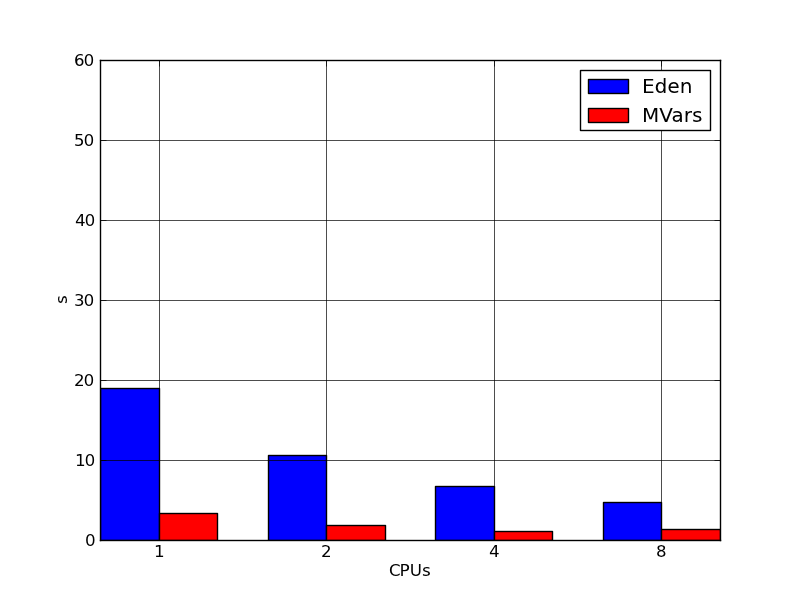
\includegraphics[width=10cm]{runtimes.png}
\end{frame}


\begin{frame}
\frametitle{Bad benchmark}

The N-body simulation benchmark from \texttt{monad-par}.

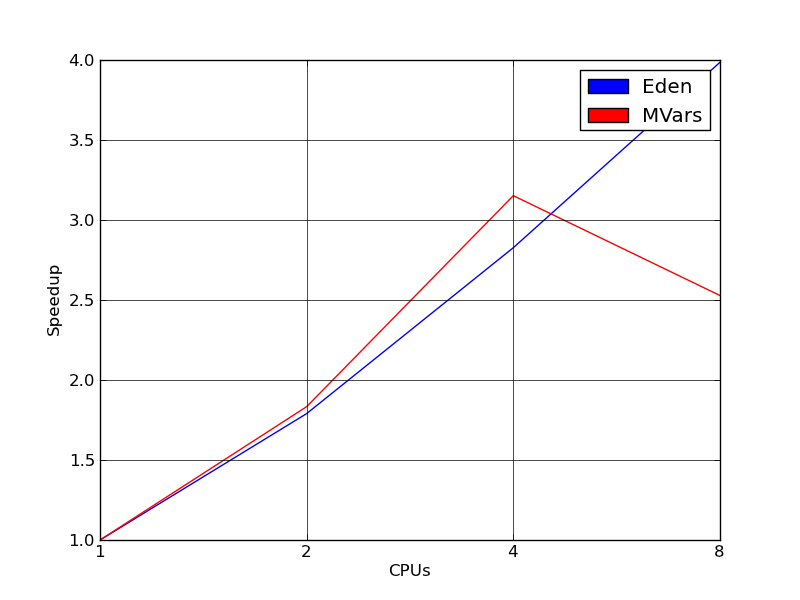
\includegraphics[width=10cm]{speedup.png}
\end{frame}

\subsection{Conclusion}

\begin{frame}
\frametitle{Conclusions}

It works, and Eden seems a good fit to the Par monad facilities.\pause

It seems to sort of scale.\pause

The implementation is still very simplistic and somewhat crude.\pause

We need a much better benchmark that shows how we can leverage a
distributed-memory cluster.

\end{frame}

\end{document}
